\section{Models}
\subsection{SZ Models}

\subsubsection{Beta Model (\betamodel)}

The \betamodel\ is an analytic shape function widely used in X-ray
analysis to fit the radial density profile:

\begin{equation}
n_e(x) = {{n_e}_0\over{\left[1 + x^2\right]^{(3\beta/2)}}}
\end{equation}

The line-integral of this function is therefore commonly used to fit the
projected 2D cluster profiles in SZ observations:

\begin{equation}
p(x) = {1\over{\left[1 + x^2\right]^{(1-3\beta/2)}}}
\end{equation}

The \betamodel\ can bs used in \climax\ by invoking \code{addmodel}
with \code{type = betamodel}.



\subsubsection{Generalized NFW (GNFW) Model}
\label{sec:gnfw}
In the context of the pressure models of \cite{nagai2007}, hereafter N07, the generalized NFW profile is given by

\begin{equation}
p(x_g) = {p_0\over{(\c500 x_g)^\gamma\left[1 + (c_{\rm 500}x_g)^\alpha\right]^{(\beta-\gamma)/\alpha}}}
\label{eq:gnfw}
\end{equation}

where $c_{\rm 500}$ is a dimensionless concentration parameter and $x_g
= r/R_{\rm 500}$.  

In \climax, the generalized NFW model is implemented as a
dimensionless shape function that can be used to fit cluster profiles
in any units:

\begin{equation}
p(x) = {1\over{x^\gamma\left[1 + x^\alpha\right]^{(\beta-\gamma)/\alpha}}}
\end{equation}

where $x = r/r_c$.  In the context of the GNFW pressure models,
therefore, the $r_c$ returned by \climax\ (actually $\theta_c$), is
equivalent to $r_c = \R500/\c500$.

The generalized NFW model can be used in \climax\ by
invoking \code{addmodel} with \code{type = gnfwmodel}.

From self-similarity arguments (see \S\ref{sec:ss}), the pressure
normalization (see Eq~\ref{eq:ytop}) of a cluster can be related to
its mass via Eq~\ref{eq:arnaud}.  In \climax\, \code{m500} can
therefore also be used with any GNFW model as the primary variable,
given a cosmology.

\subsubsection{Nagai07 GNFW Model}

N07 find that a good description of high-$T_X$ \chandra\
clusters can be fit with a model with $p_0 = 3.3$, $c_{\rm 500} = 1.8$
and $(\alpha,\beta,\gamma) = (1.3, 4.3, 0.7)$.

This specialization of the GNFW model can be used in \climax\ by
invoking \code{addmodel} with \code{type = nagai07model}.

\subsubsection{Arnaud GNFW Model}

\cite{arnaud2010}, hereafter A10, determine that $p_0 =
8.403\,h^{-3/2}_{70}$, $c_{\rm 500} = 1.17$ and $(\alpha,\beta,\gamma)
= (1.0510, 5.4905, 0.3081)$ yield the best fit to REXCESS clusters.

This specialization of the GNFW model can be used in \climax\ by
invoking \code{addmodel} with \code{type = arnaudmodel}.

A10 also determine the normalization of the pressure model fits to be

\begin{eqnarray}
P(r) &=&
1.65\times10^{-3}h(z)^{8/3}\left[{\M500\over{3\times10^{14}h^{-1}_{70}\Msolar}}\right]^{2/3+\alpha_P+\alpha^\prime_P(x)}\\\nonumber
&\times& p_{\rm A}(x_g) \,h^2_{70}\,{\rm keV\,cm^{-3}},
\end{eqnarray}

where $p_{\rm A}(x_g)$ is the GNFW profile with the Arnaud et al fit
parameters given above, $\alpha_P = 0.12$, and

\begin{equation}
\alpha^\prime_P(x_g) = 0.1 - (\alpha_P + 0.1){{(x_g/0.5)^3}\over{1 + (x_g/0.5)^3}}
\end{equation}

The small second-order $x_g$-dependent term represents a departure
from self-similarity, and also a significant increase in computational
overhead, and it is presently ignored in \climax.





\subsection{Problems with the GNFW model}
\label{sec:ss}
I have explored the GNFW model pretty extensively at this point, and
have encountered a number of issues with it:

\begin{list}{}{\labelwidth 0.4in \leftmargin \labelwidth \addtolength{\leftmargin}{\labelsep}}

\item[1] {The A10 and N07 normalizations don't agree, even for the same set of fit parameters}

\item[2] {For a given M500, the A10 normalization predicts a pressure
  (and therefore an SZ decrement) that is significantly lower than
  what we actually measure for real clusters thought to be close to that M500

  Another way of saying the same thing is that for a fixed SZ
  decrement, the GNFW model normalization predicts an M500 that is
  significantly larger than what you get from joint fits to SZ + Xray}

\item[3] {The A10 model is not self-consistent.  If you start with an
  M500 and use the A10 normalization to construct the corresponding
  pressure profile, the M500 that you get by integrating that pressure
  profile out to R500 does not agree with the M500 you started with}

\end{list}

In the next couple sections, I address each of these in turn.

\subsubsection{Comparing the A10 and N07 P500}

Substituting $f_B = 0.175, \mu = 0.59, \mu_e = 1.14, G = 6.67384\times 10^{-8} {\rm cm^{3}/(g\, s^2)}$, $h(z) \equiv H(z) / H_0$, we have

\begin{eqnarray}\nonumber
\P500 &=& {{\mu}\over{\mu_e}} f_B {{3}\over{8\pi}} \left( {{500 G^{-1/4} H(z)^2}\over{2}} \right)^{4/3}\M500^{2/3}\\\nonumber
      &=& (4197.54) \, H(z)^{8/3}\M500^{2/3}\\\nonumber
      &=& (4197.54) \, h(z)^{8/3}H_0^{8/3}\M500^{2/3}\\\nonumber
      &=& (4197.54) \, (70~{\rm km/s/Mpc})^{8/3}\,(3\times10^{14}\Msolar)^{2/3}\,h(z)^{8/3}h_{70}^{8/3}\left[{{\M500}\over{3\times10^{14}\Msolar}}\right]^{2/3}\\
      &=& 1.65\times10^{-3} \, h(z)^{8/3}h_{70}^{8/3}\left[{{\M500}\over{3\times10^{14}\Msolar}}\right]^{2/3} {\rm keV\,cm^{-3}}
\label{eq:arnaud}
\end{eqnarray}

This is to be compared to Eq~13 of A10, with which it agrees exactly.
I therefore conclude that there are no arithmetic errors in the
derivation of Arnaud's P500/M500 relationship.

Note that if we instead normalize \mathM500\ to
$1\times10^{15}\Msolar$, and take $h_{70} = 1$ or $h = 0.7$, as Nagai et al do, we
have:

\begin{equation}
\P500 = 5.89\times10^{-12} \, h(z)^{8/3}\left[{{\M500}\over{1\times10^{15}\Msolar}}\right]^{2/3} {\rm erg\,cm^{-3}}
\end{equation}

This is to be compared to Eq~3 of Nagai et al, with $h = 0.7$, which yields

\begin{equation}
\P500 = 1.14\times10^{-11} \, h(z)^{8/3}\left[{{\M500}\over{1\times10^{15}\Msolar}}\right]^{2/3} {\rm erg\,cm^{-3}}
\end{equation}

(Note that $h(z)$ is equivalent to the $E(z)$ of Nagai et al.  And N07
actually take $h = 0.72$, but I've used $h = 0.7$ for simplicity) 

The ratio of these two expressions is very close to 2, and the reason
is that N07 have dropped a factor of $h^2$ in their Eq~3, which
as-written is proportional to $h^{2/3}$ and not $h^{8/3}$, which is
clearly required by Eq~\ref{eq:p500}.  So that mystery amounts to
nothing more than typo in N07.

\subsubsection{Comparing P500 and M500}
\label{sec:confusion}

To make contact with $P_0$ of Equation~\ref{eq:ytop}, we have

\begin{eqnarray}
P_0 &=& p_0\times1.65\times10^{-3}h(z)^{8/3}\left[{\M500\over{3\times10^{14}h^{-1}_{70}\Msolar}}\right]^{2/3+\alpha_P}\,h^2_{70}\,{\rm keV\,cm^{-3}}
\label{eq:arnaudnorm}
\end{eqnarray}

(if we ignore $\alpha^\prime_P$).  This suggests, on the face of it,
that given a cosmology, we can relate an observed central decrement $y(0)$ to the Arnaud pressure normalization and therefore \mathM500\, by plugging $P_0$ into Equation~\ref{eq:ytop}.  However, I can't quite make sense of the numbers I get if I attempt to do this.  

Let's take Abell~1914 as a test case.  This cluster has a redshift $z
= 0.168$, which yields $h(z) = 1.089$ and $D_A = 0.59$~Gpc.  For A1914, the central
decrement is roughly $-2$~mK, or $y(0) \sim 4\times 10^{-4}$.  The Arnaud fits
give a typical $\theta_c\sim 2^{\,\prime}$, yielding:

\begin{equation}
P_0 = 0.29~{\rm keV/cm^3}
\end{equation}

from Equation~\ref{eq:ytop}.  Plugging the numbers into Equation~\ref{eq:arnaudnorm}, we have:

\begin{equation}
P_0 = 1.74\times 10^{-2}\left[{\M500\over{3\times10^{14}\Msolar}}\right]^{2/3+\alpha_P}~{\rm keV/cm^3},
\end{equation}

or

\begin{equation}
\M500 = 1\times10^{16}\Msolar
\end{equation}

which seems about an order of magnitude too large (estimates of the virial mass for A1914 I've seen are somewhere in the neighborhood of $2-3\times10^{15}\Msolar$).

\subsubsection{The A10 Model is not Self-consistent}

As noted above, if you start with an M500, you can use
Eq~\ref{eq:arnaud} to determine \mathP500\ and thus the normalization of
the cluster pressure profile, via Eq~\ref{eq:ytop}, in particular:

\begin{equation}\nonumber
P(r) = \P500\,p(r).
\end{equation}

where $p(r)$ is the GNFW profile in Eq~\ref{eq:gnfw}.  

This suggests that if the cluster were an isothermal sphere, then
$P(\R500)/\P500 = p(\R500) = 1.0$.  For A10's parameter values,
however, $p(\R500) = 0.48$ (which is suspiciously close to the ratio
of $(70/100)^2$).  It is also consistent with my empirical observation
that the \mathP500\ normalization predicts an SZ decrement that is
about a factor of 2 smaller than observed, for a set of clusters for
which we have independent SZ + X-ray mass estimates.

From Eq~\ref{eq:ysph} and Eq~\ref{eq:mgas} we also have:

\begin{eqnarray}
\M500 &=& {1\over{f_{gas}}}\left({{m_p\mu_e}\over{k_B T_e}}\right)\integral{\R500}{0}{P(r)}{V}\\
&=& {1\over{f_{gas}}}\left({{m_p\mu_e}\over{k_B T_e}}\right)\P500\,p_0\integral{\R500}{0}{p(r)}{V}
\end{eqnarray}

If I take measured X-ray temperatures for a set of clusters and the
A10 pressure profile fits, I can integrate this expression and
compare it to what the A10 normalization would predict for \mathM500,
and again I find that the masses I obtain in this manner are factors
of ~several lower than the best-fit \mathM500.  

All of which suggests that an appropriate way to proceed with my
simulations is to rescale $p_0$ to force self-consistency with the
input \mathM500.  That is, I find the value of $p_0$ that gives me the
same integrated \mathM500\ that I put in the model in the first place.
This factor is shown in Figure~\ref{fig:rescale}.

\begin{figure}[th]
\begin{center}
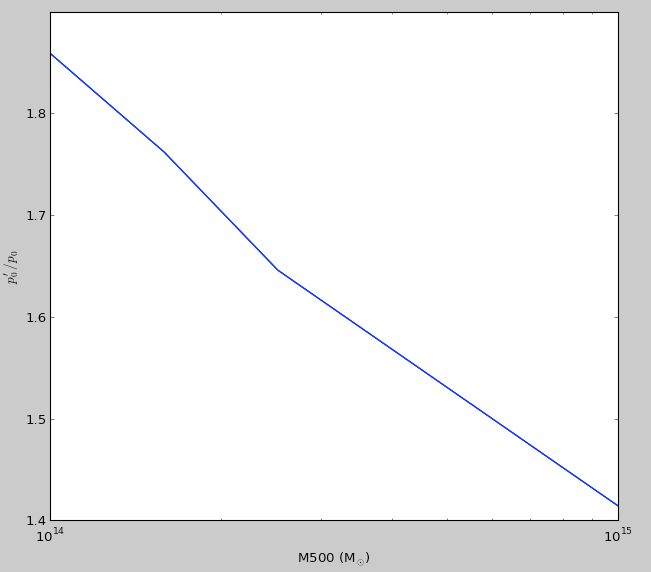
\includegraphics[scale=0.5]{figures/rescale.png}\\
\end{center}
\caption{Plot of factor by which the A10 $p_0$ needs to be rescaled to
  recover the same integrated \mathM500\ that is put into the model normalization}
\label{fig:rescale}
\end{figure}




\subsection{Other Models}

\subsubsection{Image Model}

Generic images can also be used in \climax\ as models, via
\code{adddataset} with \code{type = image}.  Supported image types,
and manipulation are as described in \S\ref{sec:imagehandling}.

Image models support only the components common to all 2D models:
translation (offsets), rotation, and scaling (normalization).  When
reading in images, you must specify either a background level, or
provide a region of the image from which it can be estimated.  This
allows for real data images to be used as models, for which a
background (i.e., constant offset) would significantly skew any
goodness-of-fit estimator.  

On read-in, this background will be subtracted from the image, and the
resulting image normalized to unity at the peak.  When comparing image
models to radio or xray data, the usual requirements for specifying
the appropriate normalization apply (i.e., \code{Sradio} or
\code{Sxray} in appropriate units).  Note that no assumptions are made
about the source of the image data; for example, if the source is an
xray surface brightness image, for example, you will probably want to
apply an appropriate transformation (i.e., \code{trans = sqrt}) to the image
before using it as an SZ model.

Currently, two operations are supported for evaluating an image model
at a requested offset, by using the \code{oper} keyword: returning the
value of the nearest pixel (\code{oper = nearest}), or interpolating
at the requested point (\code{oper = interpolate}).  For offsets that
lie outside of a model image, a zero value is returned, and the pixel
is marked as invalid.  

Invalid pixels will not be used in evaluating the likelihood for
image-plane models, however note that Fourier-plane datasets cannot
exclude individual pixels, and the zero values will be incorporated
into the transform and hence the likelihood evaluation.  You should
think carefully about what makes sense for your use-case.  Supplying a
valid image that is large enough to accomodate any offset explored by
the Markov chain can eliminate this potential problem.

An example of using an \xray-derived image model to fit SZ data is included below:

\begin{myindentpar}{3cm}
\small
\begin{verbatim}
adddataset name=sz type=uvf;
sz.file=A1914.uvf;
sz.uvmax = 2000;
sz.display = true;

addmodel name=im type=image;
im.file=acisf00542N004_cntr_img2.fits;
im.npix = 64;
im.thetaMinErr = 0.04 deg;
im.display = true;
im.interactive = true;
im.trans = sqrt;
im.sigmasmooth = 20";

im.Sradio = -2000:0 muK;
im.xoff = -0.01:0.01 deg;
im.yoff = -0.01:0.01 deg;
im.rotang = -90:90 deg;

nburn = 3000;
ntry  = 10000;

\end{verbatim}
\end{myindentpar}
